\documentclass[tikz]{standalone}
\usepackage[utf8]{inputenc}
\usepackage{tikz}
\usepackage{xcolor}
\usepackage{xcolor}
\usepackage{scalerel}
\usepackage{graphicx}
\usetikzlibrary{decorations.pathreplacing,calligraphy}
\usepackage{amsmath,amssymb,amsfonts}
\usepackage{dsfont}
\usetikzlibrary{matrix}
\usepackage{venndiagram}
\usepackage{tikz}
\usetikzlibrary{fit,shapes}

\definecolor{MyGreen}{RGB}{34,139,34}

\newcommand{\boundellipse}[3]% center, xdim, ydim
{(#1) ellipse (#2 and #3)
}

\begin{document}

%\documentclass[tikz,border=3.14mm]{standalone}



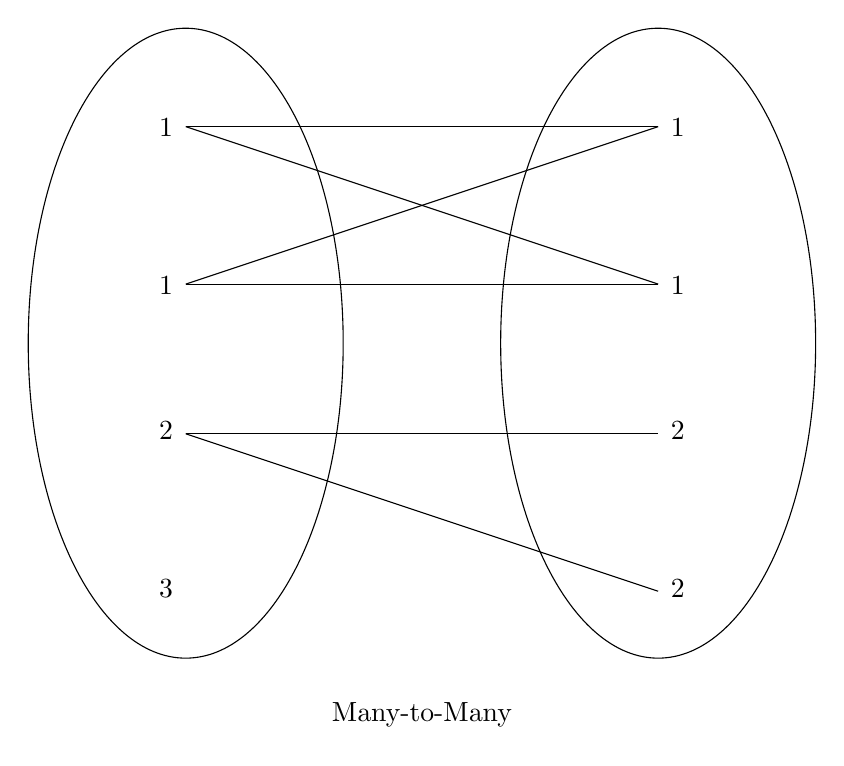
\begin{tikzpicture}

\draw \boundellipse{4,1}{-2}{4};
\draw (4, 3.75) -- (10, 3.75);
\draw (4, 3.75) -- (10, 1.75);
\draw (4, 1.75) -- (10, 3.75);
\draw (4, 1.75) -- (10, 1.75);
\draw (4, -0.15) -- (10, -0.15);
\draw (4, -0.15) -- (10, -2.15);

\draw (3.75, 3.5) node[above,align=center] {1};
\draw (3.75, 1.5) node[above,align=center] {1};
\draw (3.75, -0.35) node[above,align=center] {2};
\draw (3.75, -2.35) node[above,align=center] {3};

\draw \boundellipse{10,1}{-2}{4};


\draw (10.25, 3.5) node[above,align=center] {1};
\draw (10.25, 1.5) node[above,align=center] {1};
\draw (10.25, -0.35) node[above,align=center] {2};
\draw (10.25, -2.35) node[above,align=center] {2};

\draw (7, -4) node[above,align=center] {\text{Many-to-Many}};
\end{tikzpicture}








\end{document}


